% Options for packages loaded elsewhere
% Options for packages loaded elsewhere
\PassOptionsToPackage{unicode}{hyperref}
\PassOptionsToPackage{hyphens}{url}
\PassOptionsToPackage{dvipsnames,svgnames,x11names}{xcolor}
%
\documentclass[
  ignorenonframetext,
  aspectratio=1610,
  onlytextwidth]{beamer}
\newif\ifbibliography
\usepackage{pgfpages}
\setbeamertemplate{caption}[numbered]
\setbeamertemplate{caption label separator}{: }
\setbeamercolor{caption name}{fg=normal text.fg}
\beamertemplatenavigationsymbolsempty
% remove section numbering
\setbeamertemplate{part page}{
  \centering
  \begin{beamercolorbox}[sep=16pt,center]{part title}
    \usebeamerfont{part title}\insertpart\par
  \end{beamercolorbox}
}
\setbeamertemplate{section page}{
  \centering
  \begin{beamercolorbox}[sep=12pt,center]{section title}
    \usebeamerfont{section title}\insertsection\par
  \end{beamercolorbox}
}
\setbeamertemplate{subsection page}{
  \centering
  \begin{beamercolorbox}[sep=8pt,center]{subsection title}
    \usebeamerfont{subsection title}\insertsubsection\par
  \end{beamercolorbox}
}
% Prevent slide breaks in the middle of a paragraph
\widowpenalties 1 10000
\raggedbottom
\AtBeginPart{
  \frame{\partpage}
}
\AtBeginSection{
  \ifbibliography
  \else
    \frame{\sectionpage}
  \fi
}
\AtBeginSubsection{
  \frame{\subsectionpage}
}
\usepackage{iftex}
\ifPDFTeX
  \usepackage[T1]{fontenc}
  \usepackage[utf8]{inputenc}
  \usepackage{textcomp} % provide euro and other symbols
\else % if luatex or xetex
  \usepackage{unicode-math} % this also loads fontspec
  \defaultfontfeatures{Scale=MatchLowercase}
  \defaultfontfeatures[\rmfamily]{Ligatures=TeX,Scale=1}
\fi
\usepackage{lmodern}

\usetheme[]{moloch}
\usecolortheme[]{moloch-tomorrow}
\ifPDFTeX\else
  % xetex/luatex font selection
\fi
% Use upquote if available, for straight quotes in verbatim environments
\IfFileExists{upquote.sty}{\usepackage{upquote}}{}
\IfFileExists{microtype.sty}{% use microtype if available
  \usepackage[]{microtype}
  \UseMicrotypeSet[protrusion]{basicmath} % disable protrusion for tt fonts
}{}

\usepackage{color}
\usepackage{fancyvrb}
\newcommand{\VerbBar}{|}
\newcommand{\VERB}{\Verb[commandchars=\\\{\}]}
\DefineVerbatimEnvironment{Highlighting}{Verbatim}{commandchars=\\\{\}}
% Add ',fontsize=\small' for more characters per line
\usepackage{framed}
\definecolor{shadecolor}{RGB}{248,248,248}
\newenvironment{Shaded}{\begin{snugshade}}{\end{snugshade}}
\newcommand{\AlertTok}[1]{\textcolor[rgb]{0.94,0.16,0.16}{#1}}
\newcommand{\AnnotationTok}[1]{\textcolor[rgb]{0.56,0.35,0.01}{\textbf{\textit{#1}}}}
\newcommand{\AttributeTok}[1]{\textcolor[rgb]{0.13,0.29,0.53}{#1}}
\newcommand{\BaseNTok}[1]{\textcolor[rgb]{0.00,0.00,0.81}{#1}}
\newcommand{\BuiltInTok}[1]{#1}
\newcommand{\CharTok}[1]{\textcolor[rgb]{0.31,0.60,0.02}{#1}}
\newcommand{\CommentTok}[1]{\textcolor[rgb]{0.56,0.35,0.01}{\textit{#1}}}
\newcommand{\CommentVarTok}[1]{\textcolor[rgb]{0.56,0.35,0.01}{\textbf{\textit{#1}}}}
\newcommand{\ConstantTok}[1]{\textcolor[rgb]{0.56,0.35,0.01}{#1}}
\newcommand{\ControlFlowTok}[1]{\textcolor[rgb]{0.13,0.29,0.53}{\textbf{#1}}}
\newcommand{\DataTypeTok}[1]{\textcolor[rgb]{0.13,0.29,0.53}{#1}}
\newcommand{\DecValTok}[1]{\textcolor[rgb]{0.00,0.00,0.81}{#1}}
\newcommand{\DocumentationTok}[1]{\textcolor[rgb]{0.56,0.35,0.01}{\textbf{\textit{#1}}}}
\newcommand{\ErrorTok}[1]{\textcolor[rgb]{0.64,0.00,0.00}{\textbf{#1}}}
\newcommand{\ExtensionTok}[1]{#1}
\newcommand{\FloatTok}[1]{\textcolor[rgb]{0.00,0.00,0.81}{#1}}
\newcommand{\FunctionTok}[1]{\textcolor[rgb]{0.13,0.29,0.53}{\textbf{#1}}}
\newcommand{\ImportTok}[1]{#1}
\newcommand{\InformationTok}[1]{\textcolor[rgb]{0.56,0.35,0.01}{\textbf{\textit{#1}}}}
\newcommand{\KeywordTok}[1]{\textcolor[rgb]{0.13,0.29,0.53}{\textbf{#1}}}
\newcommand{\NormalTok}[1]{#1}
\newcommand{\OperatorTok}[1]{\textcolor[rgb]{0.81,0.36,0.00}{\textbf{#1}}}
\newcommand{\OtherTok}[1]{\textcolor[rgb]{0.56,0.35,0.01}{#1}}
\newcommand{\PreprocessorTok}[1]{\textcolor[rgb]{0.56,0.35,0.01}{\textit{#1}}}
\newcommand{\RegionMarkerTok}[1]{#1}
\newcommand{\SpecialCharTok}[1]{\textcolor[rgb]{0.81,0.36,0.00}{\textbf{#1}}}
\newcommand{\SpecialStringTok}[1]{\textcolor[rgb]{0.31,0.60,0.02}{#1}}
\newcommand{\StringTok}[1]{\textcolor[rgb]{0.31,0.60,0.02}{#1}}
\newcommand{\VariableTok}[1]{\textcolor[rgb]{0.00,0.00,0.00}{#1}}
\newcommand{\VerbatimStringTok}[1]{\textcolor[rgb]{0.31,0.60,0.02}{#1}}
\newcommand{\WarningTok}[1]{\textcolor[rgb]{0.56,0.35,0.01}{\textbf{\textit{#1}}}}

\usepackage{longtable,booktabs,array}
\usepackage{calc} % for calculating minipage widths
\usepackage{caption}
% Make caption package work with longtable
\makeatletter
\def\fnum@table{\tablename~\thetable}
\makeatother
\usepackage{graphicx}
\makeatletter
\newsavebox\pandoc@box
\newcommand*\pandocbounded[1]{% scales image to fit in text height/width
  \sbox\pandoc@box{#1}%
  \Gscale@div\@tempa{\textheight}{\dimexpr\ht\pandoc@box+\dp\pandoc@box\relax}%
  \Gscale@div\@tempb{\linewidth}{\wd\pandoc@box}%
  \ifdim\@tempb\p@<\@tempa\p@\let\@tempa\@tempb\fi% select the smaller of both
  \ifdim\@tempa\p@<\p@\scalebox{\@tempa}{\usebox\pandoc@box}%
  \else\usebox{\pandoc@box}%
  \fi%
}
% Set default figure placement to htbp
\def\fps@figure{htbp}
\makeatother





\setlength{\emergencystretch}{3em} % prevent overfull lines

\providecommand{\tightlist}{}



 


\usepackage[export]{adjustbox}
\usepackage{algorithm2e}
\usepackage{dirtree}
\setbeamertemplate{page number in head/foot}[appendixframenumber]
\setbeameroption{show notes}
\usepackage{fontsetup}
\makeatletter
\@ifpackageloaded{caption}{}{\usepackage{caption}}
\AtBeginDocument{%
\ifdefined\contentsname
  \renewcommand*\contentsname{Table of contents}
\else
  \newcommand\contentsname{Table of contents}
\fi
\ifdefined\listfigurename
  \renewcommand*\listfigurename{List of Figures}
\else
  \newcommand\listfigurename{List of Figures}
\fi
\ifdefined\listtablename
  \renewcommand*\listtablename{List of Tables}
\else
  \newcommand\listtablename{List of Tables}
\fi
\ifdefined\figurename
  \renewcommand*\figurename{Figure}
\else
  \newcommand\figurename{Figure}
\fi
\ifdefined\tablename
  \renewcommand*\tablename{Table}
\else
  \newcommand\tablename{Table}
\fi
}
\@ifpackageloaded{float}{}{\usepackage{float}}
\floatstyle{ruled}
\@ifundefined{c@chapter}{\newfloat{codelisting}{h}{lop}}{\newfloat{codelisting}{h}{lop}[chapter]}
\floatname{codelisting}{Listing}
\newcommand*\listoflistings{\listof{codelisting}{List of Listings}}
\makeatother
\makeatletter
\makeatother
\makeatletter
\@ifpackageloaded{caption}{}{\usepackage{caption}}
\@ifpackageloaded{subcaption}{}{\usepackage{subcaption}}
\makeatother

\usepackage{bookmark}
\IfFileExists{xurl.sty}{\usepackage{xurl}}{} % add URL line breaks if available
\urlstyle{same}
\hypersetup{
  pdftitle={Introduction},
  pdfauthor={Johan Larsson},
  colorlinks=true,
  linkcolor={black},
  filecolor={Maroon},
  citecolor={Blue},
  urlcolor={DodgerBlue3},
  pdfcreator={LaTeX via pandoc}}


\title{Introduction}
\subtitle{Computational Statistics}
\author{Johan Larsson}
\date{August 25, 2025}
\institute{Department of Mathematical Sciences, University of
Copenhagen}
\titlegraphic{
  
\includegraphics[right]{../images/ucph-horizontal-left.pdf}}

\begin{document}
\frame{\titlepage}


\begin{frame}{Computational Statistics?}
\phantomsection\label{computational-statistics}
\begin{columns}[T]
\begin{column}{0.47\linewidth}
\begin{block}{What Is Computational Statistics?}
\phantomsection\label{what-is-computational-statistics}
It is a broad field, where meaning depends on context.

\pause

\bipskip

One \emph{broad} definition is that it is \textbf{the use of
computational methods to solve statistical problems}, for instance

\begin{itemize}[<+->]
\tightlist
\item
  simulation,
\item
  optimization,
\item
  numerical integration,
\item
  data analysis, and
\item
  visualization.
\end{itemize}
\end{block}
\end{column}

\pause

\begin{column}{0.47\linewidth}
\begin{block}{A Running Example}
\phantomsection\label{a-running-example}
Throughout the course we will use a data set of amino acid angles,
\(\Phi\) and \(\Psi\), from protein structures.

\begin{figure}[H]

{\centering 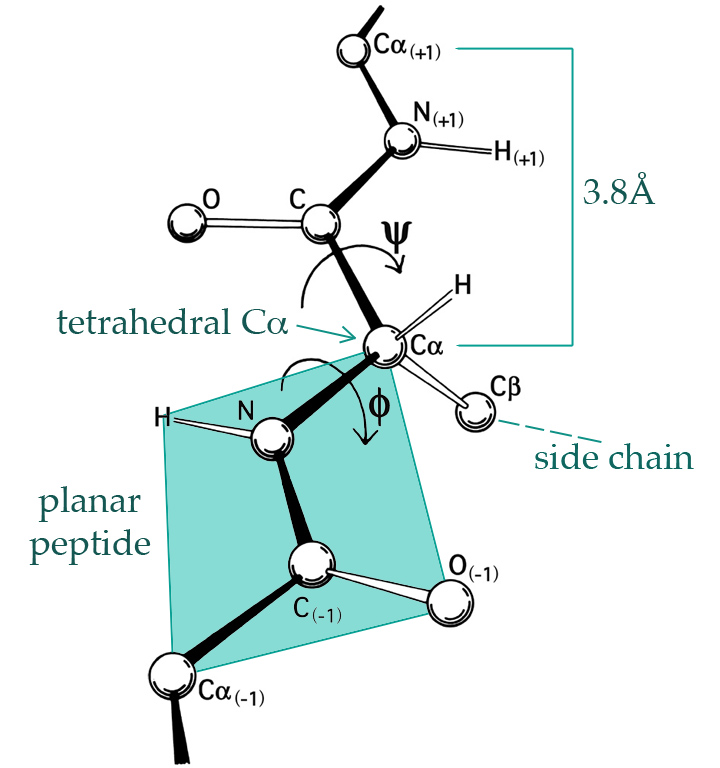
\includegraphics[width=0.7\linewidth,height=\textheight,keepaspectratio]{../images/PhiPsi_creative.jpg}

}

\caption{Amino Acid Angles}

\end{figure}%
\end{block}
\end{column}
\end{columns}
\end{frame}

\begin{frame}[fragile]{Histograms}
\phantomsection\label{histograms}
A simple way to analyze the distributions of the angles \(\Phi\) and
\(\Psi\) is the \textbf{histogram}.

\pause

\begin{columns}[T]
\begin{column}{0.47\linewidth}
\begin{Shaded}
\begin{Highlighting}[]
\FunctionTok{ggplot}\NormalTok{(phipsi, }\FunctionTok{aes}\NormalTok{(}\AttributeTok{x =}\NormalTok{ phi)) }\SpecialCharTok{+}
  \FunctionTok{geom\_histogram}\NormalTok{() }\SpecialCharTok{+}
  \FunctionTok{geom\_rug}\NormalTok{(}\AttributeTok{alpha =} \FloatTok{0.5}\NormalTok{) }\SpecialCharTok{+}
  \FunctionTok{labs}\NormalTok{(}
    \AttributeTok{x =} \FunctionTok{expression}\NormalTok{(Phi),}
    \AttributeTok{y =} \StringTok{"Density"}
\NormalTok{  )}
\end{Highlighting}
\end{Shaded}
\end{column}

\begin{column}{0.47\linewidth}
\pandocbounded{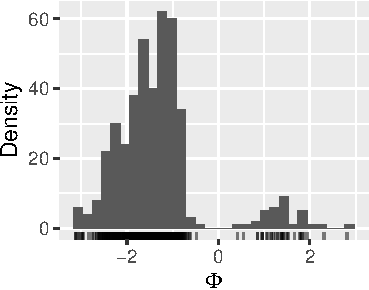
\includegraphics[keepaspectratio]{lecture1_files/figure-beamer/hist1-show-1.pdf}}
\end{column}
\end{columns}
\end{frame}

\begin{frame}[fragile]{Density Estimation}
\phantomsection\label{density-estimation}
Histograms are not very smooth. If we allow ourselves to make stronger
assumptions, we can get a smoother estimate of the distribution, using
\textbf{kernel density estimation} (KDE).

\pause

\begin{columns}[T]
\begin{column}{0.47\linewidth}
\begin{Shaded}
\begin{Highlighting}[]
\FunctionTok{ggplot}\NormalTok{(phipsi, }\FunctionTok{aes}\NormalTok{(}\AttributeTok{x =}\NormalTok{ phi)) }\SpecialCharTok{+}
  \FunctionTok{geom\_density}\NormalTok{() }\SpecialCharTok{+}
  \FunctionTok{geom\_rug}\NormalTok{(}\AttributeTok{alpha =} \FloatTok{0.5}\NormalTok{) }\SpecialCharTok{+}
  \FunctionTok{labs}\NormalTok{(}
    \AttributeTok{x =} \FunctionTok{expression}\NormalTok{(Phi),}
    \AttributeTok{y =} \StringTok{"Density"}
\NormalTok{  )}
\end{Highlighting}
\end{Shaded}
\end{column}

\begin{column}{0.47\linewidth}
\pandocbounded{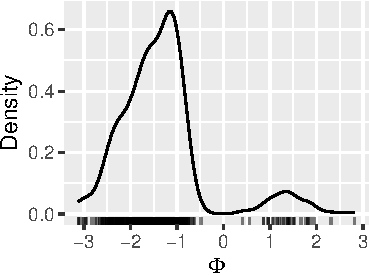
\includegraphics[keepaspectratio]{lecture1_files/figure-beamer/dens-src-1.pdf}}
\end{column}
\end{columns}

\pause

But how is this KDE actually computed? Doing this efficiently is a
\textbf{computational statistics} problem.
\end{frame}

\begin{frame}[fragile]{Statistical Topics of the Course}
\phantomsection\label{statistical-topics-of-the-course}
There are three main statistical topics of the course.

\begin{block}{Smoothing}
\phantomsection\label{smoothing}
\begin{itemize}[<+->]
\tightlist
\item
  What does \texttt{density()} do?
\item
  Nonparametric estimators
\item
  Choosing tuning parameters
\end{itemize}

\pause
\end{block}

\begin{block}{Simulation}
\phantomsection\label{simulation}
\begin{itemize}[<+->]
\tightlist
\item
  How do we efficiently simulate from a target distribution?
\item
  Assessing results from Monte Carlo methods
\item
  What if we cannot compute the density?
\end{itemize}

\pause
\end{block}

\begin{block}{Optimization}
\phantomsection\label{optimization}
\begin{itemize}[<+->]
\tightlist
\item
  How do we compute the MLE?
\item
  How to we deal with large data sets?
\end{itemize}
\end{block}
\end{frame}

\begin{frame}{Computational Topics of the Course}
\phantomsection\label{computational-topics-of-the-course}
\begin{block}{Implementation}
\phantomsection\label{implementation}
\begin{itemize}[<+->]
\tightlist
\item
  Writing functions
\item
  Object-oriented programming
\end{itemize}

\pause
\end{block}

\begin{block}{Correctness}
\phantomsection\label{correctness}
\begin{itemize}[<+->]
\tightlist
\item
  Testing
\item
  Debugging
\end{itemize}

\pause
\end{block}

\begin{block}{Efficiency}
\phantomsection\label{efficiency}
\begin{itemize}[<+->]
\tightlist
\item
  Profiling
\item
  Optimizing
\item
  Benchmarking
\end{itemize}
\end{block}
\end{frame}

\begin{frame}{Teaching Staff}
\phantomsection\label{teaching-staff}
\begin{columns}[T]
\begin{column}{0.47\linewidth}
\begin{block}{Instructor}
\phantomsection\label{instructor}
Johan Larsson, postdoctoral researcher

\begin{figure}[H]

{\centering 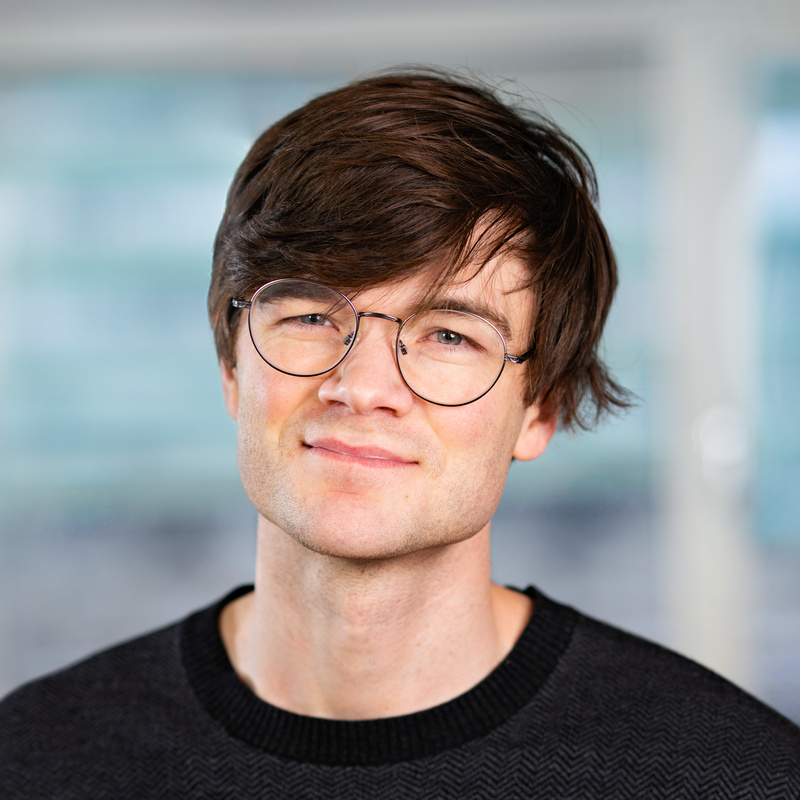
\includegraphics[width=0.5\linewidth,height=\textheight,keepaspectratio]{../images/johan.jpg}

}

\caption{Johan}

\end{figure}%

\begin{block}{Contact}
\phantomsection\label{contact}
Use Absalon for course-related questions and email (see Absalon) for
personal matters.
\end{block}
\end{block}
\end{column}

\pause

\begin{column}{0.47\linewidth}
\begin{block}{Teaching Assistant}
\phantomsection\label{teaching-assistant}
Jinyang Liu, PhD student

\begin{figure}[H]

{\centering 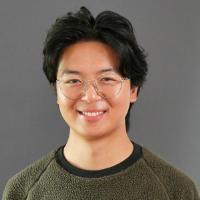
\includegraphics[width=0.5\linewidth,height=\textheight,keepaspectratio]{../images/jinyang.jpg}

}

\caption{Jin}

\end{figure}%
\end{block}
\end{column}
\end{columns}
\end{frame}

\begin{frame}{Assignments}
\phantomsection\label{assignments}
\begin{itemize}[<+->]
\tightlist
\item
  Main course work of the course
\item
  Eight assignments, two for each topic
\item
  Four topics

  \begin{itemize}[<+->]
  \tightlist
  \item
    Smoothing
  \item
    Univariate simulation
  \item
    The EM algorithm
  \item
    Stochastic optimization
  \end{itemize}
\item
  Pick one assignment per topic.
\end{itemize}
\end{frame}

\begin{frame}{Examination}
\phantomsection\label{examination}
\begin{block}{Presentations}
\phantomsection\label{presentations}
\begin{itemize}[<+->]
\tightlist
\item
  Present solution to one of the assignments.
\item
  On weeks 3, 4, 6, and 7 (Thursday afternoon sessions).
\item
  Groups of 2-3 students
\item
  Presentation, discussion, and feedback
\item
  \href{https://absalon.ku.dk/courses/76985/groups\#tab-25490}{Register
  in Absalon} (limited slots assignment)
\item
  Compulsory but not graded
\item
  Work-in-progress solutions are fine.
\end{itemize}

\pause
\end{block}

\begin{block}{Oral Examination}
\phantomsection\label{oral-examination}
\begin{itemize}[<+->]
\tightlist
\item
  Oral exam, presented indivudally.
\item
  Prepare four presentations, one for each assignment you picked.
\end{itemize}
\end{block}
\end{frame}

\begin{frame}{Schedule}
\phantomsection\label{schedule}
\begin{columns}[T]
\begin{column}{0.47\linewidth}
\begin{block}{Lectures}
\phantomsection\label{lectures}
\begin{itemize}[<+->]
\tightlist
\item
  Tuesdays and Thursdays, 10:15--12:00 (Johan)
\end{itemize}

\pause
\end{block}

\begin{block}{Exercise Sessions}
\phantomsection\label{exercise-sessions}
\begin{itemize}[<+->]
\tightlist
\item
  Thursdays, 08:15--10:00 (Jinyang)
\end{itemize}
\end{block}

\begin{block}{Presentations}
\phantomsection\label{presentations-1}
\begin{itemize}[<+->]
\tightlist
\item
  Thursdays, 13:15--15:00 (Johan)
\item
  Only weeks 3, 4, 6, and 7
\end{itemize}
\end{block}
\end{column}

\pause

\begin{column}{0.47\linewidth}
\begin{block}{Examination}
\phantomsection\label{examination-1}
\begin{itemize}[<+->]
\tightlist
\item
  November 6-8 (8.15-17.30, tentative)
\item
  Rooms to be announced
\end{itemize}
\end{block}
\end{column}
\end{columns}
\end{frame}

\begin{frame}[fragile]{Course Literature}
\phantomsection\label{course-literature}
\begin{block}{Computational Statistics with R}
\phantomsection\label{computational-statistics-with-r}
Main textbook for the course, written by Niels Richard Hansen.

\begin{itemize}[<+->]
\tightlist
\item
  Available online at \url{https://cswr.nrhstat.org/}
\item
  Not yet complete, but we only use parts that are.
\item
  \href{https://github.com/nielsrhansen/CSwR/tree/master/CSwR_package}{Companion
  package}: install with
  \texttt{pak::pak("github::nielsrhansen/CSwR/CSwR\_package")}.
\end{itemize}

\pause
\end{block}

\begin{block}{Advanced R}
\phantomsection\label{advanced-r}
Auxiliary textbook, written by Hadley Wickham.

\begin{itemize}[<+->]
\tightlist
\item
  Available online at \url{https://adv-r.hadley.nz/}
\item
  Covers more advanced R programming topics.
\item
  We will use selected chapters.
\end{itemize}
\end{block}
\end{frame}

\begin{frame}{Absalon}
\phantomsection\label{absalon}
Accessed at \href{https://absalon.ku.dk/}{absalon.ku.dk}.

\begin{columns}[T]
\begin{column}{0.47\linewidth}
\begin{itemize}[<+->]
\tightlist
\item
  \textbf{Course Material}: Slides, videos, data, groups, and
  assignments.
\item
  Actually based on Canvas (but rebranded for UCPH).
\item
  Download Canvas Student app for your phone.
\item
  Updated as we go along.
\end{itemize}
\end{column}

\begin{column}{0.47\linewidth}
\begin{figure}[H]

{\centering 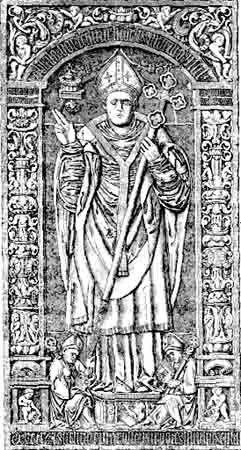
\includegraphics[width=0.5\linewidth,height=\textheight,keepaspectratio]{../images/absalon.jpg}

}

\caption{Absalon}

\end{figure}%
\end{column}
\end{columns}
\end{frame}

\begin{frame}{Generative AI}
\phantomsection\label{generative-ai}
\begin{itemize}[<+->]
\tightlist
\item
  You can use generative AI to help you with your assignments.
\item
  But you must understand the results.
\item
  Can help your learning if used correctly.
\item
  But also hamper your learning if used inappropriately (too much)
\item
  Beware of hallucinations!
\end{itemize}
\end{frame}

\section{Programming in R}\label{programming-in-r}

\begin{frame}[fragile]{Prerequisite R Knowledge}
\phantomsection\label{prerequisite-r-knowledge}
We expect knowledge of

\begin{itemize}[<+->]
\tightlist
\item
  data structures (vectors, lists, data frames),
\item
  control structures (loops, if-then-else),
\item
  function calling,
\item
  interactive and script usage (\texttt{source}) of R.
\end{itemize}

\pause

All of this is covered in chapters 1--5 of
\href{https://adv-r.hadley.nz/}{Advanced R}.

\medskip

But you \textbf{do not} need to be an experienced programmer.
\end{frame}

\section{Functions}\label{functions}

\begin{frame}[fragile]{Functions in R}
\phantomsection\label{functions-in-r}
\begin{itemize}[<+->]
\tightlist
\item
  Everything that happens in R is the result of a function call. Even
  \texttt{+}, \texttt{{[}} and \texttt{\textless{}-} are functions.
\item
  An R function takes a number of \emph{arguments}, and when a function
  call is evaluated it computes a \emph{return value}.
\item
  Functions can return any R object, including functions!
\item
  Implementations of R functions are collected into source files, which
  can be organized into packages.
\item
  The order of your functions in the script does not matter.
\end{itemize}
\end{frame}

\begin{frame}[fragile]{Components of a Function}
\phantomsection\label{components-of-a-function}
\begin{columns}[T]
\begin{column}{0.47\linewidth}
\begin{block}{Arguments}
\phantomsection\label{arguments}
\begin{Shaded}
\begin{Highlighting}[]
\NormalTok{f }\OtherTok{\textless{}{-}} \ControlFlowTok{function}\NormalTok{(x, y) \{}
\NormalTok{  x }\SpecialCharTok{+}\NormalTok{ y}
\NormalTok{\}}
\end{Highlighting}
\end{Shaded}

\pause

\begin{Shaded}
\begin{Highlighting}[]
\FunctionTok{formals}\NormalTok{(f)}
\end{Highlighting}
\end{Shaded}

\begin{verbatim}
$x


$y
\end{verbatim}
\end{block}
\end{column}

\pause

\begin{column}{0.47\linewidth}
\begin{block}{Body}
\phantomsection\label{body}
\begin{Shaded}
\begin{Highlighting}[]
\FunctionTok{body}\NormalTok{(f)}
\end{Highlighting}
\end{Shaded}

\begin{verbatim}
{
    x + y
}
\end{verbatim}

\pause
\end{block}

\begin{block}{Environment}
\phantomsection\label{environment}
\begin{Shaded}
\begin{Highlighting}[]
\FunctionTok{environment}\NormalTok{(f)}
\end{Highlighting}
\end{Shaded}

\begin{verbatim}
<environment: R_GlobalEnv>
\end{verbatim}
\end{block}
\end{column}
\end{columns}
\end{frame}

\begin{frame}[fragile]{Naming Functions}
\phantomsection\label{naming-functions}
\begin{block}{Use Descriptive Names}
\phantomsection\label{use-descriptive-names}
\begin{itemize}[<+->]
\tightlist
\item
  Verbs are great.
\item
  Better long and descriptive than short and cryptic.
\end{itemize}

\pause
\end{block}

\begin{block}{Naming Convetions}
\phantomsection\label{naming-convetions}
\begin{itemize}[<+->]
\tightlist
\item
  Avoid \texttt{.} in names; it is used for \textbf{methods} (upcoming).
\item
  Use consistent style:

  \begin{itemize}[<+->]
  \tightlist
  \item
    \texttt{lowercase}
  \item
    \texttt{snake\_case} (tidyverse)
  \item
    \texttt{camelCase}
  \item
    \texttt{UpperCamelCase}
  \end{itemize}
\end{itemize}

\pause
\end{block}

\begin{block}{Namespace Clashes}
\phantomsection\label{namespace-clashes}
\begin{itemize}[<+->]
\tightlist
\item
  Avoid names of existing functions.
\end{itemize}
\end{block}
\end{frame}

\begin{frame}[fragile]{Example: Counting Zeros}
\phantomsection\label{example-counting-zeros}
Count data is often modeled using a Poisson distribution. R can simulate
count data using the function \texttt{rpois()}.

\begin{Shaded}
\begin{Highlighting}[]
\FunctionTok{rpois}\NormalTok{(}\DecValTok{10}\NormalTok{, }\DecValTok{2}\NormalTok{) }\CommentTok{\# n = 10 variables from a Poisson(2) distribution}
\end{Highlighting}
\end{Shaded}

\begin{verbatim}
 [1] 0 2 2 2 4 2 0 1 2 2
\end{verbatim}

\pause

There are two zeros in this sequence.

\pause

Let's write a function that counts the number of zeros: checks for zero
inflation.
\end{frame}

\begin{frame}[fragile]{A First Attempt}
\phantomsection\label{a-first-attempt}
\begin{Shaded}
\begin{Highlighting}[]
\NormalTok{count\_zeros }\OtherTok{\textless{}{-}} \ControlFlowTok{function}\NormalTok{(x) \{}
\NormalTok{  n\_zeros }\OtherTok{\textless{}{-}} \DecValTok{0}
  \ControlFlowTok{for}\NormalTok{ (i }\ControlFlowTok{in} \DecValTok{1}\SpecialCharTok{:}\FunctionTok{length}\NormalTok{(x)) \{}
    \ControlFlowTok{if}\NormalTok{ (x[i] }\SpecialCharTok{==} \DecValTok{0}\NormalTok{) \{}
\NormalTok{      n\_zeros }\OtherTok{\textless{}{-}}\NormalTok{ n\_zeros }\SpecialCharTok{+} \DecValTok{1}
\NormalTok{    \}}
\NormalTok{  \}}
\NormalTok{  n\_zeros}
\NormalTok{\}}
\end{Highlighting}
\end{Shaded}

\pause

\begin{Shaded}
\begin{Highlighting}[]
\FunctionTok{count\_zeros}\NormalTok{(}\FunctionTok{c}\NormalTok{(}\DecValTok{3}\NormalTok{, }\DecValTok{2}\NormalTok{, }\DecValTok{0}\NormalTok{))}
\end{Highlighting}
\end{Shaded}

\begin{verbatim}
[1] 1
\end{verbatim}

\begin{Shaded}
\begin{Highlighting}[]
\FunctionTok{count\_zeros}\NormalTok{(}\FunctionTok{c}\NormalTok{(}\DecValTok{0}\NormalTok{, }\DecValTok{0}\NormalTok{, }\DecValTok{0}\NormalTok{))}
\end{Highlighting}
\end{Shaded}

\begin{verbatim}
[1] 3
\end{verbatim}
\end{frame}

\begin{frame}{Testing}
\phantomsection\label{testing}
\begin{itemize}[<+->]
\tightlist
\item
  Tests that a given input to a function returns what you expect.
\item
  Thumb of rule: when you find a bug in your function, write a test that
  fails on it; \emph{then} fix the function.
\item
  As you refactor your code (or dependent code changes), your tests will
  catch these \textbf{regressions} for you.
\item
  Some people even say that writing tests is the first thing you should
  do.
\item
  In R, most common solution is to use the \textbf{testthat} package.
\item
  Works best in packages, but is fine for projects too.
\end{itemize}
\end{frame}

\begin{frame}[fragile]{Testing with \textbf{testthat}}
\phantomsection\label{testing-with-testthat}
\begin{Shaded}
\begin{Highlighting}[]
\CommentTok{\# In file tests/test\_count\_zeros.R}
\FunctionTok{test\_that}\NormalTok{(}\StringTok{"count\_zeros work on various input"}\NormalTok{, \{}
  \FunctionTok{expect\_equal}\NormalTok{(}\FunctionTok{count\_zeros}\NormalTok{(}\FunctionTok{c}\NormalTok{(}\DecValTok{0}\NormalTok{, }\DecValTok{0}\NormalTok{, }\FloatTok{1e{-}9}\NormalTok{, }\DecValTok{25}\NormalTok{)), }\DecValTok{2}\NormalTok{)}
  \FunctionTok{expect\_equal}\NormalTok{(}\FunctionTok{count\_zeros}\NormalTok{(}\FunctionTok{c}\NormalTok{(}\SpecialCharTok{{-}}\DecValTok{0}\NormalTok{, }\FloatTok{1.1}\NormalTok{, }\SpecialCharTok{{-}}\DecValTok{2}\NormalTok{)), }\DecValTok{1}\NormalTok{)}
  \FunctionTok{expect\_equal}\NormalTok{(}\FunctionTok{count\_zeros}\NormalTok{(}\FunctionTok{c}\NormalTok{()), }\DecValTok{0}\NormalTok{)}
\NormalTok{\})}
\end{Highlighting}
\end{Shaded}

\begin{Shaded}
\begin{Highlighting}[]
\CommentTok{\# testthat::test\_dir("tests")}
\end{Highlighting}
\end{Shaded}
\end{frame}

\begin{frame}[fragile]{A Second Attempt}
\phantomsection\label{a-second-attempt}
\begin{Shaded}
\begin{Highlighting}[]
\NormalTok{count\_zeros }\OtherTok{\textless{}{-}} \ControlFlowTok{function}\NormalTok{(x) \{}
\NormalTok{  n\_zeros }\OtherTok{\textless{}{-}} \DecValTok{0}
  \ControlFlowTok{for}\NormalTok{ (i }\ControlFlowTok{in} \FunctionTok{seq\_along}\NormalTok{(x)) \{}
    \ControlFlowTok{if}\NormalTok{ (x[i] }\SpecialCharTok{==} \DecValTok{0}\NormalTok{) \{}
\NormalTok{      n\_zeros }\OtherTok{\textless{}{-}}\NormalTok{ n\_zeros }\SpecialCharTok{+} \DecValTok{1}
\NormalTok{    \}}
\NormalTok{  \}}
\NormalTok{  n\_zeros}
\NormalTok{\}}
\end{Highlighting}
\end{Shaded}

\begin{Shaded}
\begin{Highlighting}[]
\CommentTok{\# testthat::test\_dir("tests")}
\end{Highlighting}
\end{Shaded}
\end{frame}

\begin{frame}{Debugging}
\phantomsection\label{debugging}
\begin{itemize}[<+->]
\tightlist
\item
  Sometimes hard to identify the offending piece of code.
\item
  Helpful to use a debugging tool. R studio comes with a helpful
  interface for this.
\item
  We will talk more about debugging in week 5.
\end{itemize}
\end{frame}

\begin{frame}[fragile]{Functional Programming}
\phantomsection\label{functional-programming}
\begin{itemize}[<+->]
\tightlist
\item
  \texttt{sapply()} is what's typically called a \emph{map}, with a
  function as its second argument.
\item
  It is a feature of R as a functional programming language that it can
  operate with functions as with any other data structure.
\end{itemize}

\pause

Let's write our own apply function.

\begin{Shaded}
\begin{Highlighting}[]
\NormalTok{our\_apply }\OtherTok{\textless{}{-}} \ControlFlowTok{function}\NormalTok{(x, fun) \{}
\NormalTok{  val }\OtherTok{\textless{}{-}} \FunctionTok{numeric}\NormalTok{(}\FunctionTok{length}\NormalTok{(x)) }\CommentTok{\# initialize vector of return values}
  \ControlFlowTok{for}\NormalTok{ (i }\ControlFlowTok{in} \FunctionTok{seq\_along}\NormalTok{(x)) \{}
\NormalTok{    val[i] }\OtherTok{\textless{}{-}} \FunctionTok{fun}\NormalTok{(x[[i]])}
\NormalTok{  \}}
\NormalTok{  val}
\NormalTok{\}}
\end{Highlighting}
\end{Shaded}
\end{frame}

\begin{frame}[fragile]{Testing Our Apply Function}
\phantomsection\label{testing-our-apply-function}
\begin{Shaded}
\begin{Highlighting}[]
\FunctionTok{sapply}\NormalTok{(}\DecValTok{1}\SpecialCharTok{:}\DecValTok{10}\NormalTok{, exp)}
\end{Highlighting}
\end{Shaded}

\begin{verbatim}
 [1]     2.718282     7.389056    20.085537    54.598150   148.413159
 [6]   403.428793  1096.633158  2980.957987  8103.083928 22026.465795
\end{verbatim}

\begin{Shaded}
\begin{Highlighting}[]
\FunctionTok{our\_apply}\NormalTok{(}\DecValTok{1}\SpecialCharTok{:}\DecValTok{10}\NormalTok{, exp)}
\end{Highlighting}
\end{Shaded}

\begin{verbatim}
 [1]     2.718282     7.389056    20.085537    54.598150   148.413159
 [6]   403.428793  1096.633158  2980.957987  8103.083928 22026.465795
\end{verbatim}

\pause

\begin{block}{Assumptions}
\phantomsection\label{assumptions}
\texttt{x} is a list, \texttt{fun()} takes a single argument, and
\texttt{fun()} returns a numeric.
\end{block}
\end{frame}

\begin{frame}[fragile]{What if \texttt{fun()} Needs Additional
Arguments?}
\phantomsection\label{what-if-fun-needs-additional-arguments}
\begin{Shaded}
\begin{Highlighting}[]
\FunctionTok{our\_apply}\NormalTok{(}\DecValTok{1}\SpecialCharTok{:}\DecValTok{10}\NormalTok{, rpois)}
\end{Highlighting}
\end{Shaded}

\begin{verbatim}
Error in fun(x[[i]]): argument "lambda" is missing, with no default
\end{verbatim}

\pause

\begin{block}{Anonymous Functions}
\phantomsection\label{anonymous-functions}
\begin{Shaded}
\begin{Highlighting}[]
\FunctionTok{our\_apply}\NormalTok{(}
  \DecValTok{1}\SpecialCharTok{:}\DecValTok{10}\NormalTok{,}
  \ControlFlowTok{function}\NormalTok{(lambda) }\FunctionTok{rpois}\NormalTok{(}\DecValTok{1}\NormalTok{, }\AttributeTok{lambda =} \FloatTok{0.9}\NormalTok{)}
\NormalTok{)}
\end{Highlighting}
\end{Shaded}

\begin{verbatim}
 [1] 0 0 1 2 0 2 3 1 1 0
\end{verbatim}
\end{block}
\end{frame}

\begin{frame}[fragile]{\texttt{...}}
\phantomsection\label{section}
The \texttt{...} (ellipsis) argument passes arguments forward.

\begin{Shaded}
\begin{Highlighting}[]
\NormalTok{our\_apply }\OtherTok{\textless{}{-}} \ControlFlowTok{function}\NormalTok{(x, fun, ...) \{}
\NormalTok{  val }\OtherTok{\textless{}{-}} \FunctionTok{numeric}\NormalTok{(}\FunctionTok{length}\NormalTok{(x))}
  \ControlFlowTok{for}\NormalTok{ (i }\ControlFlowTok{in} \FunctionTok{seq\_along}\NormalTok{(x)) \{}
\NormalTok{    val[i] }\OtherTok{\textless{}{-}} \FunctionTok{fun}\NormalTok{(x[[i]], ...)}
\NormalTok{  \}}
\NormalTok{  val}
\NormalTok{\}}
\end{Highlighting}
\end{Shaded}

\pause

\begin{Shaded}
\begin{Highlighting}[]
\FunctionTok{our\_apply}\NormalTok{(}\DecValTok{1}\SpecialCharTok{:}\DecValTok{10}\NormalTok{, rpois, }\AttributeTok{n =} \DecValTok{1}\NormalTok{)}
\end{Highlighting}
\end{Shaded}

\begin{verbatim}
 [1]  0  1  4  3  7  6  8 16  8 12
\end{verbatim}
\end{frame}

\section{Benchmarking}\label{benchmarking}

\begin{frame}[fragile]{R Is Slow \ldots{}}
\phantomsection\label{r-is-slow}
\ldots{} when used like a low-level language.

\begin{itemize}[<+->]
\tightlist
\item
  R is an \textbf{interpreted} (as opposed to \emph{compiled}) language.
\item
  It was written mainly for specifying statistical models (not for
  developing new numerical methods).
\item
  It is suitable for high-level programming where most low-level
  computations are implemented in a compiled language
  (e.g.~\texttt{lm()} and \texttt{qr()}.)
\item
  It is also quite old.
\end{itemize}
\end{frame}

\begin{frame}[fragile]{R Is Fast \ldots{}}
\phantomsection\label{r-is-fast}
\ldots{} when most computations are carried out by calls to compiled
code.

\begin{Shaded}
\begin{Highlighting}[]
\NormalTok{x }\OtherTok{\textless{}{-}} \FunctionTok{rnorm}\NormalTok{(}\FloatTok{1e4}\NormalTok{)}
\NormalTok{bench\_res }\OtherTok{\textless{}{-}}\NormalTok{ bench}\SpecialCharTok{::}\FunctionTok{mark}\NormalTok{(}
\NormalTok{  \{}
\NormalTok{    y }\OtherTok{\textless{}{-}} \FunctionTok{numeric}\NormalTok{(}\FunctionTok{length}\NormalTok{(x))}
    \ControlFlowTok{for}\NormalTok{ (i }\ControlFlowTok{in} \FunctionTok{seq\_along}\NormalTok{(x)) \{}
\NormalTok{      y[i] }\OtherTok{\textless{}{-}} \DecValTok{10} \SpecialCharTok{*}\NormalTok{ x[i]}
\NormalTok{    \}}
\NormalTok{    y}
\NormalTok{  \},}
  \DecValTok{10} \SpecialCharTok{*}\NormalTok{ x}
\NormalTok{)}
\end{Highlighting}
\end{Shaded}
\end{frame}

\begin{frame}[fragile]{Plot Benchmark Results}
\phantomsection\label{plot-benchmark-results}
\begin{Shaded}
\begin{Highlighting}[]
\FunctionTok{autoplot}\NormalTok{(bench\_res)}
\end{Highlighting}
\end{Shaded}

\pandocbounded{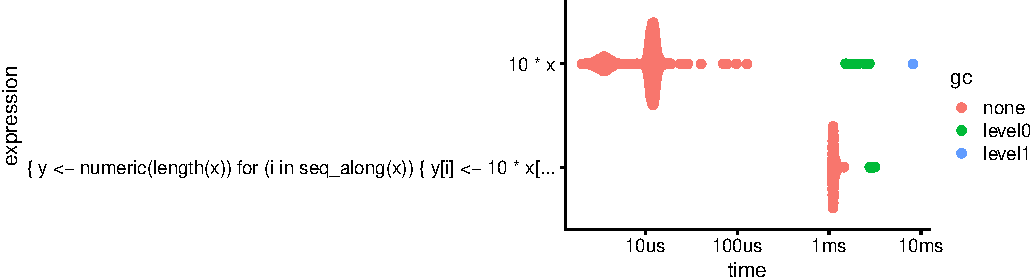
\includegraphics[keepaspectratio]{lecture1_files/figure-beamer/bench-plot-1.pdf}}
\end{frame}

\begin{frame}[fragile]{Beware of Loops in Disguise}
\phantomsection\label{beware-of-loops-in-disguise}
Just because you ran a function, it does not mean that it is vectorized.

\pause

\begin{Shaded}
\begin{Highlighting}[]
\NormalTok{bench}\SpecialCharTok{::}\FunctionTok{mark}\NormalTok{(}
  \FunctionTok{sapply}\NormalTok{(x, }\ControlFlowTok{function}\NormalTok{(x\_i) }\DecValTok{10} \SpecialCharTok{*}\NormalTok{ x\_i),}
  \DecValTok{10} \SpecialCharTok{*}\NormalTok{ x}
\NormalTok{) }\SpecialCharTok{|\textgreater{}}
  \FunctionTok{plot}\NormalTok{()}
\end{Highlighting}
\end{Shaded}

\pandocbounded{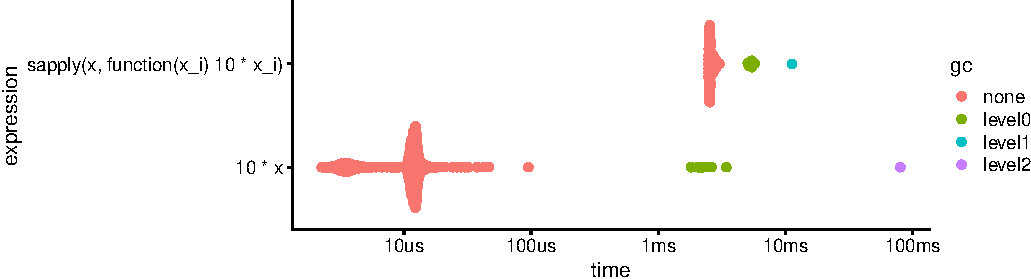
\includegraphics[keepaspectratio]{lecture1_files/figure-beamer/unnamed-chunk-16-1.pdf}}
\end{frame}

\begin{frame}[fragile]{Vectorization}
\phantomsection\label{vectorization}
\begin{Shaded}
\begin{Highlighting}[]
\NormalTok{count\_zeros\_vec }\OtherTok{\textless{}{-}} \ControlFlowTok{function}\NormalTok{(x) \{}
  \FunctionTok{sum}\NormalTok{(x }\SpecialCharTok{==} \DecValTok{0}\NormalTok{)}
\NormalTok{\}}
\end{Highlighting}
\end{Shaded}

\pause

\begin{itemize}[<+->]
\tightlist
\item
  \texttt{x\ ==\ 0} checks if each entry of \texttt{x} is 0 and returns
  a vector of logicals.
\item
  \texttt{sum()} computes and returns the sum of all elements in a
  vector. Logicals are coerced to integers.
\item
  In this case the vectorized implementation is cohesive and clear.
\item
  The vectorized computations are performed by compiled code
  (C/C++/Fortran), which run faster than pure R code.
\item
  Writing vectorized code requires a larger knowledge of R functions.
\end{itemize}
\end{frame}

\begin{frame}{Development Cycle Sketch}
\phantomsection\label{development-cycle-sketch}
\begin{itemize}[<+->]
\tightlist
\item
  Is there a good-enough existing implemention for your problem? If yes,
  then you are done.
\item
  If not, implement a solution and test it. Does it solve your problem
  sufficiently well? If yes, then you're done.
\item
  If not, then profile (next week!), benchmark, and debug (week 5). Then
  refactor and optimize.
\end{itemize}

\pause

\begin{block}{The Root of All Evil}
\phantomsection\label{the-root-of-all-evil}
\medskip

\begin{quote}
We \emph{should} forget about small efficiencies, say about 97\% of the
time: premature optimization is the root of all evil. Yet we should not
pass up our opportunities in that critical 3\%.

\emph{---Donald Knuth}
\end{quote}
\end{block}
\end{frame}

\begin{frame}[fragile]{Example: Density Estimation}
\phantomsection\label{example-density-estimation}
\begin{Shaded}
\begin{Highlighting}[]
\NormalTok{kern\_dens }\OtherTok{\textless{}{-}} \ControlFlowTok{function}\NormalTok{(x, h, }\AttributeTok{m =} \DecValTok{512}\NormalTok{) \{}
\NormalTok{  rg }\OtherTok{\textless{}{-}} \FunctionTok{range}\NormalTok{(x)}
\NormalTok{  xx }\OtherTok{\textless{}{-}} \FunctionTok{seq}\NormalTok{(rg[}\DecValTok{1}\NormalTok{] }\SpecialCharTok{{-}} \DecValTok{3} \SpecialCharTok{*}\NormalTok{ h, rg[}\DecValTok{2}\NormalTok{] }\SpecialCharTok{+} \DecValTok{3} \SpecialCharTok{*}\NormalTok{ h, }\AttributeTok{length.out =}\NormalTok{ m)}
\NormalTok{  y }\OtherTok{\textless{}{-}} \FunctionTok{numeric}\NormalTok{(m)}

  \ControlFlowTok{for}\NormalTok{ (i }\ControlFlowTok{in} \FunctionTok{seq\_along}\NormalTok{(xx)) \{}
    \ControlFlowTok{for}\NormalTok{ (j }\ControlFlowTok{in} \FunctionTok{seq\_along}\NormalTok{(x)) \{}
\NormalTok{      y[i] }\OtherTok{\textless{}{-}}\NormalTok{ y[i] }\SpecialCharTok{+} \FunctionTok{exp}\NormalTok{(}\SpecialCharTok{{-}}\NormalTok{(xx[i] }\SpecialCharTok{{-}}\NormalTok{ x[j])}\SpecialCharTok{\^{}}\DecValTok{2} \SpecialCharTok{/}\NormalTok{ (}\DecValTok{2} \SpecialCharTok{*}\NormalTok{ h}\SpecialCharTok{\^{}}\DecValTok{2}\NormalTok{))}
\NormalTok{    \}}
\NormalTok{  \}}

\NormalTok{  y }\OtherTok{\textless{}{-}}\NormalTok{ y }\SpecialCharTok{/}\NormalTok{ (}\FunctionTok{sqrt}\NormalTok{(}\DecValTok{2} \SpecialCharTok{*}\NormalTok{ pi) }\SpecialCharTok{*}\NormalTok{ h }\SpecialCharTok{*} \FunctionTok{length}\NormalTok{(x))}

  \FunctionTok{list}\NormalTok{(}\AttributeTok{x =}\NormalTok{ xx, }\AttributeTok{y =}\NormalTok{ y)}
\NormalTok{\}}
\end{Highlighting}
\end{Shaded}
\end{frame}

\begin{frame}[fragile]{Vectorizing Our Density Estimator}
\phantomsection\label{vectorizing-our-density-estimator}
\begin{Shaded}
\begin{Highlighting}[]
\NormalTok{kern\_dens\_vec }\OtherTok{\textless{}{-}} \ControlFlowTok{function}\NormalTok{(x, h, }\AttributeTok{m =} \DecValTok{512}\NormalTok{) \{}
\NormalTok{  rg }\OtherTok{\textless{}{-}} \FunctionTok{range}\NormalTok{(x)}
\NormalTok{  xx }\OtherTok{\textless{}{-}} \FunctionTok{seq}\NormalTok{(rg[}\DecValTok{1}\NormalTok{] }\SpecialCharTok{{-}} \DecValTok{3} \SpecialCharTok{*}\NormalTok{ h, rg[}\DecValTok{2}\NormalTok{] }\SpecialCharTok{+} \DecValTok{3} \SpecialCharTok{*}\NormalTok{ h, }\AttributeTok{length.out =}\NormalTok{ m)}
\NormalTok{  y }\OtherTok{\textless{}{-}} \FunctionTok{numeric}\NormalTok{(m)}
\NormalTok{  const }\OtherTok{\textless{}{-}}\NormalTok{ (}\FunctionTok{sqrt}\NormalTok{(}\DecValTok{2} \SpecialCharTok{*}\NormalTok{ pi) }\SpecialCharTok{*}\NormalTok{ h }\SpecialCharTok{*} \FunctionTok{length}\NormalTok{(x))}

  \ControlFlowTok{for}\NormalTok{ (i }\ControlFlowTok{in} \FunctionTok{seq\_along}\NormalTok{(xx)) \{}
\NormalTok{    y[i] }\OtherTok{\textless{}{-}} \FunctionTok{sum}\NormalTok{(}\FunctionTok{exp}\NormalTok{(}\SpecialCharTok{{-}}\NormalTok{(xx[i] }\SpecialCharTok{{-}}\NormalTok{ x)}\SpecialCharTok{\^{}}\DecValTok{2} \SpecialCharTok{/}\NormalTok{ (}\DecValTok{2} \SpecialCharTok{*}\NormalTok{ h}\SpecialCharTok{\^{}}\DecValTok{2}\NormalTok{))) }\SpecialCharTok{/}\NormalTok{ const}
\NormalTok{  \}}

  \FunctionTok{list}\NormalTok{(}\AttributeTok{x =}\NormalTok{ xx, }\AttributeTok{y =}\NormalTok{ y)}
\NormalTok{\}}
\end{Highlighting}
\end{Shaded}
\end{frame}

\begin{frame}[fragile]{Benchmarking}
\phantomsection\label{benchmarking-1}
\begin{Shaded}
\begin{Highlighting}[]
\NormalTok{kern\_bench }\OtherTok{\textless{}{-}}\NormalTok{ bench}\SpecialCharTok{::}\FunctionTok{mark}\NormalTok{(}
  \FunctionTok{kern\_dens}\NormalTok{(phipsi}\SpecialCharTok{$}\NormalTok{psi, }\FloatTok{0.2}\NormalTok{),}
  \FunctionTok{kern\_dens\_vec}\NormalTok{(phipsi}\SpecialCharTok{$}\NormalTok{psi, }\FloatTok{0.2}\NormalTok{)}
\NormalTok{)}

\FunctionTok{summary}\NormalTok{(kern\_bench)}
\end{Highlighting}
\end{Shaded}

\begin{verbatim}
# A tibble: 2 x 6
  expression                          min   median `itr/sec` mem_alloc `gc/sec`
  <bch:expr>                     <bch:tm> <bch:tm>     <dbl> <bch:byt>    <dbl>
1 kern_dens(phipsi$psi, 0.2)      13.61ms  13.65ms      72.9        NA      0  
2 kern_dens_vec(phipsi$psi, 0.2)   1.17ms   1.21ms     812.         NA     26.5
\end{verbatim}
\end{frame}

\begin{frame}[fragile]{Plot Benchmark Results}
\phantomsection\label{plot-benchmark-results-1}
\begin{Shaded}
\begin{Highlighting}[]
\FunctionTok{plot}\NormalTok{(kern\_bench, }\AttributeTok{type =} \StringTok{"violin"}\NormalTok{)}
\end{Highlighting}
\end{Shaded}

\pandocbounded{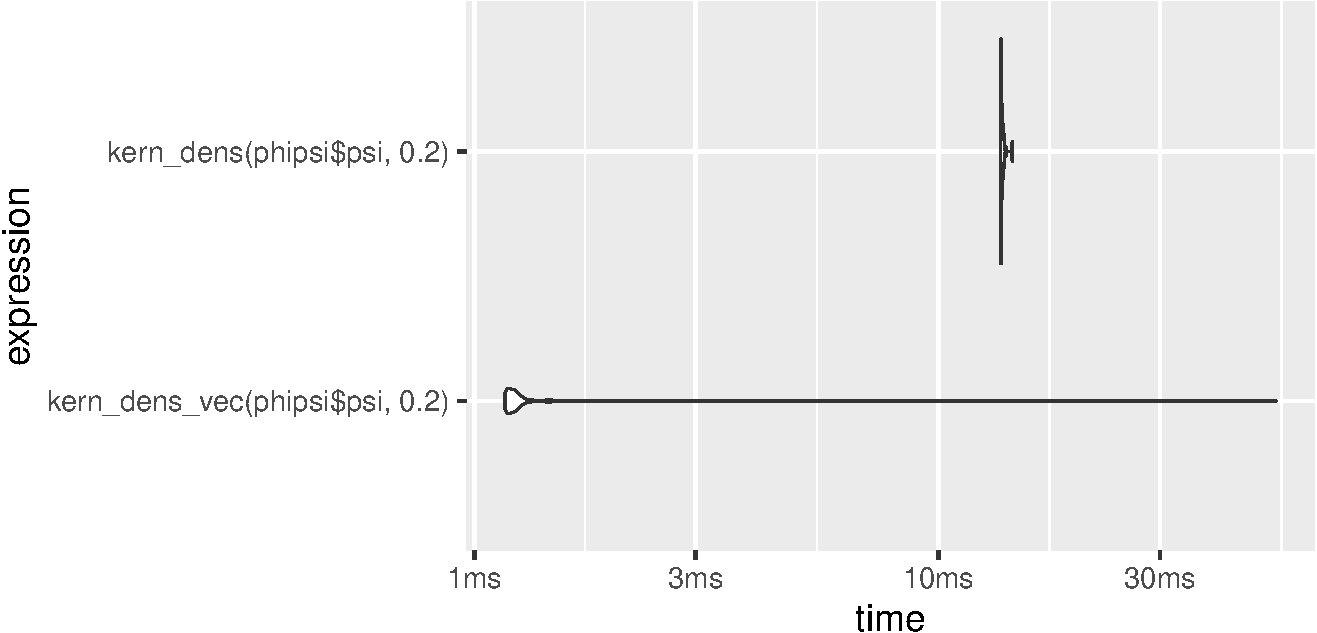
\includegraphics[keepaspectratio]{lecture1_files/figure-beamer/kern-bench-autoplot-1.pdf}}
\end{frame}

\begin{frame}[fragile]{Parameterized Benchmarking}
\phantomsection\label{parameterized-benchmarking}
\begin{Shaded}
\begin{Highlighting}[]
\NormalTok{kern\_benchmarks }\OtherTok{\textless{}{-}}\NormalTok{ bench}\SpecialCharTok{::}\FunctionTok{press}\NormalTok{(}
  \AttributeTok{n =} \DecValTok{2}\SpecialCharTok{\^{}}\NormalTok{(}\DecValTok{6}\SpecialCharTok{:}\DecValTok{9}\NormalTok{),}
  \AttributeTok{m =} \DecValTok{2}\SpecialCharTok{\^{}}\NormalTok{(}\DecValTok{5}\SpecialCharTok{:}\DecValTok{11}\NormalTok{),}
\NormalTok{  \{}
\NormalTok{    bench}\SpecialCharTok{::}\FunctionTok{mark}\NormalTok{(}
      \AttributeTok{loop =} \FunctionTok{kern\_dens}\NormalTok{(x[}\DecValTok{1}\SpecialCharTok{:}\NormalTok{n], }\AttributeTok{h =} \FloatTok{0.2}\NormalTok{, }\AttributeTok{m =}\NormalTok{ m),}
      \AttributeTok{vec =} \FunctionTok{kern\_dens\_vec}\NormalTok{(x[}\DecValTok{1}\SpecialCharTok{:}\NormalTok{n], }\AttributeTok{h =} \FloatTok{0.2}\NormalTok{, }\AttributeTok{m =}\NormalTok{ m)}
\NormalTok{    )}
\NormalTok{  \}}
\NormalTok{)}
\end{Highlighting}
\end{Shaded}
\end{frame}

\begin{frame}[fragile]{Plotting Results}
\phantomsection\label{plotting-results}
\begin{Shaded}
\begin{Highlighting}[]
\FunctionTok{library}\NormalTok{(tidyverse)}
\FunctionTok{mutate}\NormalTok{(kern\_benchmarks, }\AttributeTok{expression =} \FunctionTok{as.character}\NormalTok{(expression)) }\SpecialCharTok{|\textgreater{}}
  \FunctionTok{ggplot}\NormalTok{(}\FunctionTok{aes}\NormalTok{(m, median, }\AttributeTok{color =}\NormalTok{ expression)) }\SpecialCharTok{+}
  \FunctionTok{geom\_point}\NormalTok{() }\SpecialCharTok{+}
  \FunctionTok{geom\_line}\NormalTok{() }\SpecialCharTok{+}
  \FunctionTok{facet\_grid}\NormalTok{(}\AttributeTok{cols =} \FunctionTok{vars}\NormalTok{(n))}
\end{Highlighting}
\end{Shaded}

\pandocbounded{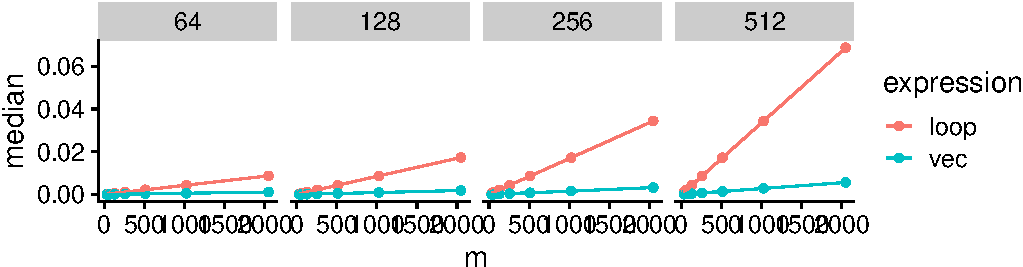
\includegraphics[keepaspectratio]{lecture1_files/figure-beamer/kern-bench-fig-1.pdf}}
\end{frame}

\begin{frame}{Getting Help with R}
\phantomsection\label{getting-help-with-r}
\begin{block}{Google It}
\phantomsection\label{google-it}
Especially good for error messages.

\pause
\end{block}

\begin{block}{Generative AI}
\phantomsection\label{generative-ai-1}
\begin{itemize}[<+->]
\tightlist
\item
  Also great for error messages and debugging
\item
  \emph{Caution}: You need to understand the results, especially when
  you ask it to create something for you.
\end{itemize}

\pause
\end{block}

\begin{block}{Absalon Discussion Forum}
\phantomsection\label{absalon-discussion-forum}
Use the fact that there are twenty other people in the course with
exactly the same problem.
\end{block}
\end{frame}

\section{Exercises}\label{exercises}

\begin{frame}[fragile]{Exercises}
\begin{block}{Exercise 1}
\phantomsection\label{exercise-1}
Can you list three ways to access element \texttt{a} in this list?

\begin{Shaded}
\begin{Highlighting}[]
\NormalTok{l }\OtherTok{\textless{}{-}} \FunctionTok{list}\NormalTok{(}\AttributeTok{a =} \DecValTok{1}\NormalTok{, }\AttributeTok{b =} \DecValTok{2}\NormalTok{)}
\end{Highlighting}
\end{Shaded}

\pause
\end{block}

\begin{block}{Exercise 2}
\phantomsection\label{exercise-2}
Write a for loop that prints ``even'' if the loop variable is even,
``odd'' if the loop variable is odd, and exits if is larger than 10.
\end{block}
\end{frame}




\end{document}
